\documentclass[twoside]{book}

% Packages required by doxygen
\usepackage{fixltx2e}
\usepackage{calc}
\usepackage{doxygen}
\usepackage[export]{adjustbox} % also loads graphicx
\usepackage{graphicx}
\usepackage[utf8]{inputenc}
\usepackage{makeidx}
\usepackage{multicol}
\usepackage{multirow}
\PassOptionsToPackage{warn}{textcomp}
\usepackage{textcomp}
\usepackage[nointegrals]{wasysym}
\usepackage[table]{xcolor}

% Font selection
\usepackage[T1]{fontenc}
\usepackage[scaled=.90]{helvet}
\usepackage{courier}
\usepackage{amssymb}
\usepackage{sectsty}
\renewcommand{\familydefault}{\sfdefault}
\allsectionsfont{%
  \fontseries{bc}\selectfont%
  \color{darkgray}%
}
\renewcommand{\DoxyLabelFont}{%
  \fontseries{bc}\selectfont%
  \color{darkgray}%
}
\newcommand{\+}{\discretionary{\mbox{\scriptsize$\hookleftarrow$}}{}{}}

% Page & text layout
\usepackage{geometry}
\geometry{%
  a4paper,%
  top=2.5cm,%
  bottom=2.5cm,%
  left=2.5cm,%
  right=2.5cm%
}
\tolerance=750
\hfuzz=15pt
\hbadness=750
\setlength{\emergencystretch}{15pt}
\setlength{\parindent}{0cm}
\setlength{\parskip}{3ex plus 2ex minus 2ex}
\makeatletter
\renewcommand{\paragraph}{%
  \@startsection{paragraph}{4}{0ex}{-1.0ex}{1.0ex}{%
    \normalfont\normalsize\bfseries\SS@parafont%
  }%
}
\renewcommand{\subparagraph}{%
  \@startsection{subparagraph}{5}{0ex}{-1.0ex}{1.0ex}{%
    \normalfont\normalsize\bfseries\SS@subparafont%
  }%
}
\makeatother

% Headers & footers
\usepackage{fancyhdr}
\pagestyle{fancyplain}
\fancyhead[LE]{\fancyplain{}{\bfseries\thepage}}
\fancyhead[CE]{\fancyplain{}{}}
\fancyhead[RE]{\fancyplain{}{\bfseries\leftmark}}
\fancyhead[LO]{\fancyplain{}{\bfseries\rightmark}}
\fancyhead[CO]{\fancyplain{}{}}
\fancyhead[RO]{\fancyplain{}{\bfseries\thepage}}
\fancyfoot[LE]{\fancyplain{}{}}
\fancyfoot[CE]{\fancyplain{}{}}
\fancyfoot[RE]{\fancyplain{}{\bfseries\scriptsize Generated by Doxygen }}
\fancyfoot[LO]{\fancyplain{}{\bfseries\scriptsize Generated by Doxygen }}
\fancyfoot[CO]{\fancyplain{}{}}
\fancyfoot[RO]{\fancyplain{}{}}
\renewcommand{\footrulewidth}{0.4pt}
\renewcommand{\chaptermark}[1]{%
  \markboth{#1}{}%
}
\renewcommand{\sectionmark}[1]{%
  \markright{\thesection\ #1}%
}

% Indices & bibliography
\usepackage{natbib}
\usepackage[titles]{tocloft}
\setcounter{tocdepth}{3}
\setcounter{secnumdepth}{5}
\makeindex

% Hyperlinks (required, but should be loaded last)
\usepackage{ifpdf}
\ifpdf
  \usepackage[pdftex,pagebackref=true]{hyperref}
\else
  \usepackage[ps2pdf,pagebackref=true]{hyperref}
\fi
\hypersetup{%
  colorlinks=true,%
  linkcolor=blue,%
  citecolor=blue,%
  unicode%
}

% Custom commands
\newcommand{\clearemptydoublepage}{%
  \newpage{\pagestyle{empty}\cleardoublepage}%
}

\usepackage{caption}
\captionsetup{labelsep=space,justification=centering,font={bf},singlelinecheck=off,skip=4pt,position=top}

%===== C O N T E N T S =====

\begin{document}

% Titlepage & ToC
\hypersetup{pageanchor=false,
             bookmarksnumbered=true,
             pdfencoding=unicode
            }
\pagenumbering{alph}
\begin{titlepage}
\vspace*{7cm}
\begin{center}%
{\Large My Project }\\
\vspace*{1cm}
{\large Generated by Doxygen 1.8.13}\\
\end{center}
\end{titlepage}
\clearemptydoublepage
\pagenumbering{roman}
\tableofcontents
\clearemptydoublepage
\pagenumbering{arabic}
\hypersetup{pageanchor=true}

%--- Begin generated contents ---
\chapter{Hierarchical Index}
\section{Class Hierarchy}
This inheritance list is sorted roughly, but not completely, alphabetically\+:\begin{DoxyCompactList}
\item \contentsline{section}{Chmod\+Props}{\pageref{structChmodProps}}{}
\item \contentsline{section}{Content}{\pageref{structContent}}{}
\item \contentsline{section}{Dir\+Block}{\pageref{structDirBlock}}{}
\item \contentsline{section}{disk\+\_\+commands}{\pageref{classdisk__commands}}{}
\item \contentsline{section}{Disk\+Commands\+Props}{\pageref{structDiskCommandsProps}}{}
\item \contentsline{section}{E\+BR}{\pageref{structEBR}}{}
\item \contentsline{section}{File\+Block}{\pageref{structFileBlock}}{}
\item \contentsline{section}{graph\+\_\+commands}{\pageref{classgraph__commands}}{}
\item \contentsline{section}{group\+\_\+commands}{\pageref{classgroup__commands}}{}
\item \contentsline{section}{Inode}{\pageref{structInode}}{}
\item \contentsline{section}{Journal}{\pageref{structJournal}}{}
\item \contentsline{section}{List\+Prop}{\pageref{structListProp}}{}
\item \contentsline{section}{M\+BR}{\pageref{structMBR}}{}
\item \contentsline{section}{Mk\+User\+Props}{\pageref{structMkUserProps}}{}
\item \contentsline{section}{Mounted\+Partition}{\pageref{structMountedPartition}}{}
\item \contentsline{section}{node\+\_\+commands}{\pageref{classnode__commands}}{}
\item \contentsline{section}{Partition}{\pageref{structPartition}}{}
\item \contentsline{section}{partition\+\_\+commands}{\pageref{classpartition__commands}}{}
\item \contentsline{section}{Partition\+Commands\+Props}{\pageref{structPartitionCommandsProps}}{}
\item \contentsline{section}{Partition\+Fs\+Props}{\pageref{structPartitionFsProps}}{}
\item \contentsline{section}{permission\+\_\+commands}{\pageref{classpermission__commands}}{}
\item \contentsline{section}{Prop\+Variant}{\pageref{structPropVariant}}{}
\item \contentsline{section}{Rep\+Props}{\pageref{structRepProps}}{}
\item \contentsline{section}{Super\+Block}{\pageref{structSuperBlock}}{}
\item \contentsline{section}{Touch\+Props}{\pageref{structTouchProps}}{}
\item \contentsline{section}{user\+\_\+commands}{\pageref{classuser__commands}}{}
\item \contentsline{section}{User\+Commands\+Props}{\pageref{structUserCommandsProps}}{}
\begin{DoxyCompactList}
\item \contentsline{section}{User}{\pageref{structUser}}{}
\end{DoxyCompactList}
\item \contentsline{section}{User\+Or\+Group}{\pageref{structUserOrGroup}}{}
\item \contentsline{section}{yy\+\_\+buffer\+\_\+state}{\pageref{structyy__buffer__state}}{}
\item \contentsline{section}{yy\+\_\+trans\+\_\+info}{\pageref{structyy__trans__info}}{}
\item \contentsline{section}{yyalloc}{\pageref{unionyyalloc}}{}
\item \contentsline{section}{Y\+Y\+L\+T\+Y\+PE}{\pageref{structYYLTYPE}}{}
\item \contentsline{section}{Y\+Y\+S\+T\+Y\+PE}{\pageref{unionYYSTYPE}}{}
\end{DoxyCompactList}

\chapter{Class Index}
\section{Class List}
Here are the classes, structs, unions and interfaces with brief descriptions\+:\begin{DoxyCompactList}
\item\contentsline{section}{\hyperlink{structChmodProps}{Chmod\+Props} }{\pageref{structChmodProps}}{}
\item\contentsline{section}{\hyperlink{structContent}{Content} }{\pageref{structContent}}{}
\item\contentsline{section}{\hyperlink{structDirBlock}{Dir\+Block} }{\pageref{structDirBlock}}{}
\item\contentsline{section}{\hyperlink{classdisk__commands}{disk\+\_\+commands} }{\pageref{classdisk__commands}}{}
\item\contentsline{section}{\hyperlink{structDiskCommandsProps}{Disk\+Commands\+Props} }{\pageref{structDiskCommandsProps}}{}
\item\contentsline{section}{\hyperlink{structEBR}{E\+BR} }{\pageref{structEBR}}{}
\item\contentsline{section}{\hyperlink{structFileBlock}{File\+Block} }{\pageref{structFileBlock}}{}
\item\contentsline{section}{\hyperlink{classgraph__commands}{graph\+\_\+commands} }{\pageref{classgraph__commands}}{}
\item\contentsline{section}{\hyperlink{classgroup__commands}{group\+\_\+commands} }{\pageref{classgroup__commands}}{}
\item\contentsline{section}{\hyperlink{structInode}{Inode} }{\pageref{structInode}}{}
\item\contentsline{section}{\hyperlink{structJournal}{Journal} }{\pageref{structJournal}}{}
\item\contentsline{section}{\hyperlink{structListProp}{List\+Prop} }{\pageref{structListProp}}{}
\item\contentsline{section}{\hyperlink{structMBR}{M\+BR} }{\pageref{structMBR}}{}
\item\contentsline{section}{\hyperlink{structMkUserProps}{Mk\+User\+Props} }{\pageref{structMkUserProps}}{}
\item\contentsline{section}{\hyperlink{structMountedPartition}{Mounted\+Partition} }{\pageref{structMountedPartition}}{}
\item\contentsline{section}{\hyperlink{classnode__commands}{node\+\_\+commands} }{\pageref{classnode__commands}}{}
\item\contentsline{section}{\hyperlink{structPartition}{Partition} }{\pageref{structPartition}}{}
\item\contentsline{section}{\hyperlink{classpartition__commands}{partition\+\_\+commands} }{\pageref{classpartition__commands}}{}
\item\contentsline{section}{\hyperlink{structPartitionCommandsProps}{Partition\+Commands\+Props} }{\pageref{structPartitionCommandsProps}}{}
\item\contentsline{section}{\hyperlink{structPartitionFsProps}{Partition\+Fs\+Props} }{\pageref{structPartitionFsProps}}{}
\item\contentsline{section}{\hyperlink{classpermission__commands}{permission\+\_\+commands} }{\pageref{classpermission__commands}}{}
\item\contentsline{section}{\hyperlink{structPropVariant}{Prop\+Variant} }{\pageref{structPropVariant}}{}
\item\contentsline{section}{\hyperlink{structRepProps}{Rep\+Props} }{\pageref{structRepProps}}{}
\item\contentsline{section}{\hyperlink{structSuperBlock}{Super\+Block} }{\pageref{structSuperBlock}}{}
\item\contentsline{section}{\hyperlink{structTouchProps}{Touch\+Props} }{\pageref{structTouchProps}}{}
\item\contentsline{section}{\hyperlink{structUser}{User} }{\pageref{structUser}}{}
\item\contentsline{section}{\hyperlink{classuser__commands}{user\+\_\+commands} }{\pageref{classuser__commands}}{}
\item\contentsline{section}{\hyperlink{structUserCommandsProps}{User\+Commands\+Props} }{\pageref{structUserCommandsProps}}{}
\item\contentsline{section}{\hyperlink{structUserOrGroup}{User\+Or\+Group} }{\pageref{structUserOrGroup}}{}
\item\contentsline{section}{\hyperlink{structyy__buffer__state}{yy\+\_\+buffer\+\_\+state} }{\pageref{structyy__buffer__state}}{}
\item\contentsline{section}{\hyperlink{structyy__trans__info}{yy\+\_\+trans\+\_\+info} }{\pageref{structyy__trans__info}}{}
\item\contentsline{section}{\hyperlink{unionyyalloc}{yyalloc} }{\pageref{unionyyalloc}}{}
\item\contentsline{section}{\hyperlink{structYYLTYPE}{Y\+Y\+L\+T\+Y\+PE} }{\pageref{structYYLTYPE}}{}
\item\contentsline{section}{\hyperlink{unionYYSTYPE}{Y\+Y\+S\+T\+Y\+PE} }{\pageref{unionYYSTYPE}}{}
\end{DoxyCompactList}

\chapter{Class Documentation}
\hypertarget{structChmodProps}{}\section{Chmod\+Props Struct Reference}
\label{structChmodProps}\index{Chmod\+Props@{Chmod\+Props}}
\subsection*{Public Member Functions}
\begin{DoxyCompactItemize}
\item 
\mbox{\Hypertarget{structChmodProps_a08772639aee06f98492670051a86fe9b}\label{structChmodProps_a08772639aee06f98492670051a86fe9b}} 
void {\bfseries set\+\_\+prop} (string value, string key)
\end{DoxyCompactItemize}
\subsection*{Public Attributes}
\begin{DoxyCompactItemize}
\item 
\mbox{\Hypertarget{structChmodProps_aecb787e1ca110239b753a6cc48c21c51}\label{structChmodProps_aecb787e1ca110239b753a6cc48c21c51}} 
bool {\bfseries recursive} = 0
\item 
\mbox{\Hypertarget{structChmodProps_a21f3211be6f8a92b571fc97997144748}\label{structChmodProps_a21f3211be6f8a92b571fc97997144748}} 
string {\bfseries path}
\item 
\mbox{\Hypertarget{structChmodProps_a9d4abcc6c05af2e100ea9eae2c5864d5}\label{structChmodProps_a9d4abcc6c05af2e100ea9eae2c5864d5}} 
string {\bfseries ugo}
\end{DoxyCompactItemize}


The documentation for this struct was generated from the following file\+:\begin{DoxyCompactItemize}
\item 
permissions/index.\+h\end{DoxyCompactItemize}

\hypertarget{structContent}{}\section{Content Struct Reference}
\label{structContent}\index{Content@{Content}}
\subsection*{Public Attributes}
\begin{DoxyCompactItemize}
\item 
\mbox{\Hypertarget{structContent_ab53e9e33f352e8f5cc4b0fa4aea82a03}\label{structContent_ab53e9e33f352e8f5cc4b0fa4aea82a03}} 
char {\bfseries name} \mbox{[}12\mbox{]}
\item 
\mbox{\Hypertarget{structContent_a39332cd745caaeff2667e564c1220adf}\label{structContent_a39332cd745caaeff2667e564c1220adf}} 
int {\bfseries inodo}
\end{DoxyCompactItemize}


The documentation for this struct was generated from the following file\+:\begin{DoxyCompactItemize}
\item 
partitions/index.\+h\end{DoxyCompactItemize}

\hypertarget{structDirBlock}{}\section{Dir\+Block Struct Reference}
\label{structDirBlock}\index{Dir\+Block@{Dir\+Block}}


Collaboration diagram for Dir\+Block\+:\nopagebreak
\begin{figure}[H]
\begin{center}
\leavevmode
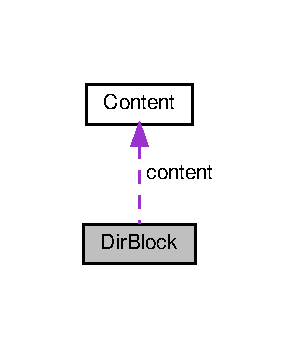
\includegraphics[width=143pt]{structDirBlock__coll__graph}
\end{center}
\end{figure}
\subsection*{Public Attributes}
\begin{DoxyCompactItemize}
\item 
\mbox{\Hypertarget{structDirBlock_a3d5fd85614aa8242ad3d49dcff2ac784}\label{structDirBlock_a3d5fd85614aa8242ad3d49dcff2ac784}} 
\hyperlink{structContent}{Content} {\bfseries content} \mbox{[}4\mbox{]}
\end{DoxyCompactItemize}


The documentation for this struct was generated from the following file\+:\begin{DoxyCompactItemize}
\item 
partitions/index.\+h\end{DoxyCompactItemize}

\hypertarget{classdisk__commands}{}\section{disk\+\_\+commands Class Reference}
\label{classdisk__commands}\index{disk\+\_\+commands@{disk\+\_\+commands}}
\subsection*{Public Member Functions}
\begin{DoxyCompactItemize}
\item 
void \hyperlink{classdisk__commands_a5a447276c75f649b6fef291ac05c053f}{mkdisk} (\hyperlink{structDiskCommandsProps}{Disk\+Commands\+Props} props)
\begin{DoxyCompactList}\small\item\em Crea un disco vacio con 4 particiones. \end{DoxyCompactList}\item 
void \hyperlink{classdisk__commands_aaa2145946615ccf353aea1380a6a8e7e}{rmdisk} (string path)
\begin{DoxyCompactList}\small\item\em Borra el archivo .disk. \end{DoxyCompactList}\end{DoxyCompactItemize}


\subsection{Member Function Documentation}
\mbox{\Hypertarget{classdisk__commands_a5a447276c75f649b6fef291ac05c053f}\label{classdisk__commands_a5a447276c75f649b6fef291ac05c053f}} 
\index{disk\+\_\+commands@{disk\+\_\+commands}!mkdisk@{mkdisk}}
\index{mkdisk@{mkdisk}!disk\+\_\+commands@{disk\+\_\+commands}}
\subsubsection{\texorpdfstring{mkdisk()}{mkdisk()}}
{\footnotesize\ttfamily void disk\+\_\+commands\+::mkdisk (\begin{DoxyParamCaption}\item[{\hyperlink{structDiskCommandsProps}{Disk\+Commands\+Props}}]{props }\end{DoxyParamCaption})}



Crea un disco vacio con 4 particiones. 

Crear disco 
\begin{DoxyParams}{Parameters}
{\em \{\+Disk\+Commands\+Props\}} & disk\+\_\+data \\
\hline
\end{DoxyParams}
\mbox{\Hypertarget{classdisk__commands_aaa2145946615ccf353aea1380a6a8e7e}\label{classdisk__commands_aaa2145946615ccf353aea1380a6a8e7e}} 
\index{disk\+\_\+commands@{disk\+\_\+commands}!rmdisk@{rmdisk}}
\index{rmdisk@{rmdisk}!disk\+\_\+commands@{disk\+\_\+commands}}
\subsubsection{\texorpdfstring{rmdisk()}{rmdisk()}}
{\footnotesize\ttfamily void disk\+\_\+commands\+::rmdisk (\begin{DoxyParamCaption}\item[{string}]{path }\end{DoxyParamCaption})}



Borra el archivo .disk. 

Borrar disco 
\begin{DoxyParams}{Parameters}
{\em \{string\}} & path \\
\hline
\end{DoxyParams}


The documentation for this class was generated from the following files\+:\begin{DoxyCompactItemize}
\item 
disks/index.\+h\item 
disks/index.\+cpp\end{DoxyCompactItemize}

\hypertarget{structDiskCommandsProps}{}\section{Disk\+Commands\+Props Struct Reference}
\label{structDiskCommandsProps}\index{Disk\+Commands\+Props@{Disk\+Commands\+Props}}
\subsection*{Public Member Functions}
\begin{DoxyCompactItemize}
\item 
\mbox{\Hypertarget{structDiskCommandsProps_ab747ea0dd5ac4b327a12fee7474f4723}\label{structDiskCommandsProps_ab747ea0dd5ac4b327a12fee7474f4723}} 
void {\bfseries set\+\_\+prop} (string value, string name)
\end{DoxyCompactItemize}
\subsection*{Public Attributes}
\begin{DoxyCompactItemize}
\item 
\mbox{\Hypertarget{structDiskCommandsProps_ad81ed25cc8e07974a918fe78f4849da6}\label{structDiskCommandsProps_ad81ed25cc8e07974a918fe78f4849da6}} 
char {\bfseries unit} = \textquotesingle{}M\textquotesingle{}
\item 
\mbox{\Hypertarget{structDiskCommandsProps_af12962b744838d683f7b8025c0aac8a5}\label{structDiskCommandsProps_af12962b744838d683f7b8025c0aac8a5}} 
char {\bfseries fit} = \textquotesingle{}F\textquotesingle{}
\item 
\mbox{\Hypertarget{structDiskCommandsProps_adc6e22a84d4d91b937d7ba60934fcf5f}\label{structDiskCommandsProps_adc6e22a84d4d91b937d7ba60934fcf5f}} 
string {\bfseries path} = \char`\"{}\char`\"{}
\item 
\mbox{\Hypertarget{structDiskCommandsProps_adfa30ea70cf9fddd5731e54444d633e6}\label{structDiskCommandsProps_adfa30ea70cf9fddd5731e54444d633e6}} 
int {\bfseries size} = -\/1
\end{DoxyCompactItemize}


The documentation for this struct was generated from the following file\+:\begin{DoxyCompactItemize}
\item 
disks/index.\+h\end{DoxyCompactItemize}

\hypertarget{structEBR}{}\section{E\+BR Struct Reference}
\label{structEBR}\index{E\+BR@{E\+BR}}
\subsection*{Public Attributes}
\begin{DoxyCompactItemize}
\item 
\mbox{\Hypertarget{structEBR_a424b668c478fb095f726e4931e671e6f}\label{structEBR_a424b668c478fb095f726e4931e671e6f}} 
char {\bfseries name} \mbox{[}16\mbox{]}
\item 
\mbox{\Hypertarget{structEBR_a7e8263addb859bc2e3ec7997c937dddc}\label{structEBR_a7e8263addb859bc2e3ec7997c937dddc}} 
char {\bfseries status}
\item 
\mbox{\Hypertarget{structEBR_aff99ac49b8abf7396e9ca61fd0682003}\label{structEBR_aff99ac49b8abf7396e9ca61fd0682003}} 
int {\bfseries start}
\item 
\mbox{\Hypertarget{structEBR_afe72f9429195e6995a62db9f5e5190cc}\label{structEBR_afe72f9429195e6995a62db9f5e5190cc}} 
char {\bfseries fit}
\item 
\mbox{\Hypertarget{structEBR_a83a7e6369f07cb2ed71b69c9c887c427}\label{structEBR_a83a7e6369f07cb2ed71b69c9c887c427}} 
int {\bfseries size}
\item 
\mbox{\Hypertarget{structEBR_a2b166e9d7ed9d1011a1792f246915b54}\label{structEBR_a2b166e9d7ed9d1011a1792f246915b54}} 
int {\bfseries next}
\end{DoxyCompactItemize}


The documentation for this struct was generated from the following file\+:\begin{DoxyCompactItemize}
\item 
disks/index.\+h\end{DoxyCompactItemize}

\hypertarget{structFileBlock}{}\section{File\+Block Struct Reference}
\label{structFileBlock}\index{File\+Block@{File\+Block}}
\subsection*{Public Attributes}
\begin{DoxyCompactItemize}
\item 
\mbox{\Hypertarget{structFileBlock_a39884276ea655ff94d8f378968a1c57d}\label{structFileBlock_a39884276ea655ff94d8f378968a1c57d}} 
char {\bfseries content} \mbox{[}64\mbox{]}
\end{DoxyCompactItemize}


The documentation for this struct was generated from the following file\+:\begin{DoxyCompactItemize}
\item 
partitions/index.\+h\end{DoxyCompactItemize}

\hypertarget{classgraph__commands}{}\section{graph\+\_\+commands Class Reference}
\label{classgraph__commands}\index{graph\+\_\+commands@{graph\+\_\+commands}}
\subsection*{Public Member Functions}
\begin{DoxyCompactItemize}
\item 
void \hyperlink{classgraph__commands_a0b916a2e77374903ea346ff795521487}{rep} (\hyperlink{structRepProps}{Rep\+Props} props)
\begin{DoxyCompactList}\small\item\em Generar reportes de todo tipo. \end{DoxyCompactList}\end{DoxyCompactItemize}


\subsection{Member Function Documentation}
\mbox{\Hypertarget{classgraph__commands_a0b916a2e77374903ea346ff795521487}\label{classgraph__commands_a0b916a2e77374903ea346ff795521487}} 
\index{graph\+\_\+commands@{graph\+\_\+commands}!rep@{rep}}
\index{rep@{rep}!graph\+\_\+commands@{graph\+\_\+commands}}
\subsubsection{\texorpdfstring{rep()}{rep()}}
{\footnotesize\ttfamily void graph\+\_\+commands\+::rep (\begin{DoxyParamCaption}\item[{\hyperlink{structRepProps}{Rep\+Props}}]{props }\end{DoxyParamCaption})}



Generar reportes de todo tipo. 

Reportes 
\begin{DoxyParams}{Parameters}
{\em props} & \\
\hline
\end{DoxyParams}


The documentation for this class was generated from the following files\+:\begin{DoxyCompactItemize}
\item 
graphs/index.\+h\item 
graphs/index.\+cpp\end{DoxyCompactItemize}

\hypertarget{classgroup__commands}{}\section{group\+\_\+commands Class Reference}
\label{classgroup__commands}\index{group\+\_\+commands@{group\+\_\+commands}}
\subsection*{Public Member Functions}
\begin{DoxyCompactItemize}
\item 
void \hyperlink{classgroup__commands_a333c1ce212ad3c9f24692eec6c6b8c12}{mkgrp} (string name)
\begin{DoxyCompactList}\small\item\em Crea un grupo en una particion. \end{DoxyCompactList}\item 
void \hyperlink{classgroup__commands_acc331b882e646298ca4c3ff4678ff34c}{rmgrp} (string name)
\begin{DoxyCompactList}\small\item\em Configura el id 0 para el grupo seleccioando. \end{DoxyCompactList}\end{DoxyCompactItemize}


\subsection{Member Function Documentation}
\mbox{\Hypertarget{classgroup__commands_a333c1ce212ad3c9f24692eec6c6b8c12}\label{classgroup__commands_a333c1ce212ad3c9f24692eec6c6b8c12}} 
\index{group\+\_\+commands@{group\+\_\+commands}!mkgrp@{mkgrp}}
\index{mkgrp@{mkgrp}!group\+\_\+commands@{group\+\_\+commands}}
\subsubsection{\texorpdfstring{mkgrp()}{mkgrp()}}
{\footnotesize\ttfamily void group\+\_\+commands\+::mkgrp (\begin{DoxyParamCaption}\item[{string}]{name }\end{DoxyParamCaption})}



Crea un grupo en una particion. 

Crear grupo 
\begin{DoxyParams}{Parameters}
{\em \{string\}} & name \\
\hline
\end{DoxyParams}
\mbox{\Hypertarget{classgroup__commands_acc331b882e646298ca4c3ff4678ff34c}\label{classgroup__commands_acc331b882e646298ca4c3ff4678ff34c}} 
\index{group\+\_\+commands@{group\+\_\+commands}!rmgrp@{rmgrp}}
\index{rmgrp@{rmgrp}!group\+\_\+commands@{group\+\_\+commands}}
\subsubsection{\texorpdfstring{rmgrp()}{rmgrp()}}
{\footnotesize\ttfamily void group\+\_\+commands\+::rmgrp (\begin{DoxyParamCaption}\item[{string}]{name }\end{DoxyParamCaption})}



Configura el id 0 para el grupo seleccioando. 

Borrar grupo 
\begin{DoxyParams}{Parameters}
{\em \{string\}} & name \\
\hline
\end{DoxyParams}


The documentation for this class was generated from the following files\+:\begin{DoxyCompactItemize}
\item 
groups/index.\+h\item 
groups/index.\+cpp\end{DoxyCompactItemize}

\hypertarget{structInode}{}\section{Inode Struct Reference}
\label{structInode}\index{Inode@{Inode}}
\subsection*{Public Attributes}
\begin{DoxyCompactItemize}
\item 
\mbox{\Hypertarget{structInode_a1a0b7a2d0eacf3384ceacc30b5339fd5}\label{structInode_a1a0b7a2d0eacf3384ceacc30b5339fd5}} 
char {\bfseries atime} \mbox{[}17\mbox{]}
\item 
\mbox{\Hypertarget{structInode_ac824acd449fcc512c5486fc5ed355f75}\label{structInode_ac824acd449fcc512c5486fc5ed355f75}} 
char {\bfseries ctime} \mbox{[}17\mbox{]}
\item 
\mbox{\Hypertarget{structInode_a0d7889b8ff6317ed4c11073dffba0ddd}\label{structInode_a0d7889b8ff6317ed4c11073dffba0ddd}} 
char {\bfseries mtime} \mbox{[}17\mbox{]}
\item 
\mbox{\Hypertarget{structInode_ad00b0133f27b92819fc56dc833bf31c7}\label{structInode_ad00b0133f27b92819fc56dc833bf31c7}} 
int {\bfseries block} \mbox{[}15\mbox{]}
\item 
\mbox{\Hypertarget{structInode_a742789b80d71e963d3bd98c6d4704a5a}\label{structInode_a742789b80d71e963d3bd98c6d4704a5a}} 
char {\bfseries type}
\item 
\mbox{\Hypertarget{structInode_a222a216233050983f2f7b6c8ccbdce71}\label{structInode_a222a216233050983f2f7b6c8ccbdce71}} 
int {\bfseries size}
\item 
\mbox{\Hypertarget{structInode_a96bd0c95097c57c5133b457fbd93d362}\label{structInode_a96bd0c95097c57c5133b457fbd93d362}} 
int {\bfseries perm}
\item 
\mbox{\Hypertarget{structInode_acf389c19512ceb25e8e624dca171164c}\label{structInode_acf389c19512ceb25e8e624dca171164c}} 
int {\bfseries uid}
\item 
\mbox{\Hypertarget{structInode_a5d8f156e89ab3700e17246750c176716}\label{structInode_a5d8f156e89ab3700e17246750c176716}} 
int {\bfseries gid}
\end{DoxyCompactItemize}


The documentation for this struct was generated from the following file\+:\begin{DoxyCompactItemize}
\item 
partitions/index.\+h\end{DoxyCompactItemize}

\hypertarget{structJournal}{}\section{Journal Struct Reference}
\label{structJournal}\index{Journal@{Journal}}
\subsection*{Public Attributes}
\begin{DoxyCompactItemize}
\item 
\mbox{\Hypertarget{structJournal_a0c80567e2226e83ba4600ba1864de8bf}\label{structJournal_a0c80567e2226e83ba4600ba1864de8bf}} 
char {\bfseries operation} \mbox{[}10\mbox{]}
\item 
\mbox{\Hypertarget{structJournal_abcc17172cb9f9a050cb4af67c592d869}\label{structJournal_abcc17172cb9f9a050cb4af67c592d869}} 
char {\bfseries content} \mbox{[}200\mbox{]}
\item 
\mbox{\Hypertarget{structJournal_aa888e32b3a06e48f51029ef7965794f0}\label{structJournal_aa888e32b3a06e48f51029ef7965794f0}} 
int {\bfseries permissions}
\item 
\mbox{\Hypertarget{structJournal_af567a68495575d14ee9c37d8eca93019}\label{structJournal_af567a68495575d14ee9c37d8eca93019}} 
char {\bfseries name} \mbox{[}200\mbox{]}
\item 
\mbox{\Hypertarget{structJournal_a754c3b3c833b9ea2dc797f6ed7a5d8c8}\label{structJournal_a754c3b3c833b9ea2dc797f6ed7a5d8c8}} 
char {\bfseries owner} \mbox{[}10\mbox{]}
\item 
\mbox{\Hypertarget{structJournal_abd46b33cecbdccf990c475af712fac82}\label{structJournal_abd46b33cecbdccf990c475af712fac82}} 
char {\bfseries date} \mbox{[}17\mbox{]}
\item 
\mbox{\Hypertarget{structJournal_ae5d57aaa0d6e5dd4a60a4d359e449833}\label{structJournal_ae5d57aaa0d6e5dd4a60a4d359e449833}} 
char {\bfseries type}
\end{DoxyCompactItemize}


The documentation for this struct was generated from the following file\+:\begin{DoxyCompactItemize}
\item 
partitions/index.\+h\end{DoxyCompactItemize}

\hypertarget{structListProp}{}\section{List\+Prop Struct Reference}
\label{structListProp}\index{List\+Prop@{List\+Prop}}
\subsection*{Public Attributes}
\begin{DoxyCompactItemize}
\item 
\mbox{\Hypertarget{structListProp_a198f5e2593758a78e31b4ae777839ce6}\label{structListProp_a198f5e2593758a78e31b4ae777839ce6}} 
vector$<$ string $>$ {\bfseries list}
\end{DoxyCompactItemize}


The documentation for this struct was generated from the following file\+:\begin{DoxyCompactItemize}
\item 
nodes/index.\+h\end{DoxyCompactItemize}

\hypertarget{structMBR}{}\section{M\+BR Struct Reference}
\label{structMBR}\index{M\+BR@{M\+BR}}


Collaboration diagram for M\+BR\+:\nopagebreak
\begin{figure}[H]
\begin{center}
\leavevmode
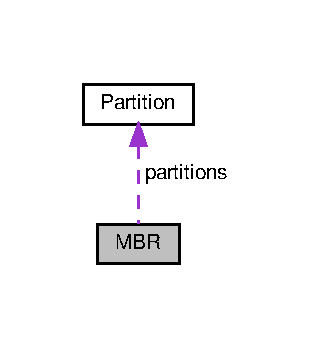
\includegraphics[width=149pt]{structMBR__coll__graph}
\end{center}
\end{figure}
\subsection*{Public Attributes}
\begin{DoxyCompactItemize}
\item 
\mbox{\Hypertarget{structMBR_aeb9fb3879f3fe8f907e4da6926807c39}\label{structMBR_aeb9fb3879f3fe8f907e4da6926807c39}} 
\hyperlink{structPartition}{Partition} {\bfseries partitions} \mbox{[}4\mbox{]}
\item 
\mbox{\Hypertarget{structMBR_ab2c49558e385fffabd122d10137f100a}\label{structMBR_ab2c49558e385fffabd122d10137f100a}} 
char {\bfseries date} \mbox{[}17\mbox{]}
\item 
\mbox{\Hypertarget{structMBR_a95adb1d5b9f1b47d9c2f8d1280eef7ab}\label{structMBR_a95adb1d5b9f1b47d9c2f8d1280eef7ab}} 
int {\bfseries signature}
\item 
\mbox{\Hypertarget{structMBR_a4ea809a4b447f6c7bb9f37835b0d42c7}\label{structMBR_a4ea809a4b447f6c7bb9f37835b0d42c7}} 
char {\bfseries fit}
\item 
\mbox{\Hypertarget{structMBR_ab66bd5bedf898f05b844d19cb1b31134}\label{structMBR_ab66bd5bedf898f05b844d19cb1b31134}} 
int {\bfseries size}
\end{DoxyCompactItemize}


The documentation for this struct was generated from the following file\+:\begin{DoxyCompactItemize}
\item 
disks/index.\+h\end{DoxyCompactItemize}

\hypertarget{structMkUserProps}{}\section{Mk\+User\+Props Struct Reference}
\label{structMkUserProps}\index{Mk\+User\+Props@{Mk\+User\+Props}}
\subsection*{Public Member Functions}
\begin{DoxyCompactItemize}
\item 
\mbox{\Hypertarget{structMkUserProps_a88f46764ef6961838a5e1e2c3f9cb1e6}\label{structMkUserProps_a88f46764ef6961838a5e1e2c3f9cb1e6}} 
void {\bfseries set\+\_\+prop} (string value, string key)
\end{DoxyCompactItemize}
\subsection*{Public Attributes}
\begin{DoxyCompactItemize}
\item 
\mbox{\Hypertarget{structMkUserProps_affa4c6a7223e3b99ab81cf9cce734f8a}\label{structMkUserProps_affa4c6a7223e3b99ab81cf9cce734f8a}} 
string {\bfseries usr}
\item 
\mbox{\Hypertarget{structMkUserProps_a0bd374781644c54fa0912eeeb475697f}\label{structMkUserProps_a0bd374781644c54fa0912eeeb475697f}} 
string {\bfseries pwd}
\item 
\mbox{\Hypertarget{structMkUserProps_af5ebdee0dbf515f4eb0532ce17a3a93a}\label{structMkUserProps_af5ebdee0dbf515f4eb0532ce17a3a93a}} 
string {\bfseries grp}
\end{DoxyCompactItemize}


The documentation for this struct was generated from the following file\+:\begin{DoxyCompactItemize}
\item 
users/index.\+h\end{DoxyCompactItemize}

\hypertarget{structMountedPartition}{}\section{Mounted\+Partition Struct Reference}
\label{structMountedPartition}\index{Mounted\+Partition@{Mounted\+Partition}}
\subsection*{Public Attributes}
\begin{DoxyCompactItemize}
\item 
\mbox{\Hypertarget{structMountedPartition_aab3bd309dbb4a176fa2f23c850fa68d9}\label{structMountedPartition_aab3bd309dbb4a176fa2f23c850fa68d9}} 
string {\bfseries name}
\item 
\mbox{\Hypertarget{structMountedPartition_a3458bbf0240918c6b0fd247ee0c3405e}\label{structMountedPartition_a3458bbf0240918c6b0fd247ee0c3405e}} 
string {\bfseries path}
\item 
\mbox{\Hypertarget{structMountedPartition_a74a74c123c693156aad8b7a840aeac7c}\label{structMountedPartition_a74a74c123c693156aad8b7a840aeac7c}} 
char {\bfseries type}
\item 
\mbox{\Hypertarget{structMountedPartition_a88f48e09db3ebc627c09351ad525a5ab}\label{structMountedPartition_a88f48e09db3ebc627c09351ad525a5ab}} 
string {\bfseries id}
\item 
\mbox{\Hypertarget{structMountedPartition_a5f05f2067502eef644a8b8076ccef89a}\label{structMountedPartition_a5f05f2067502eef644a8b8076ccef89a}} 
int {\bfseries start}
\item 
\mbox{\Hypertarget{structMountedPartition_ad462d68d54c5bbab2e1f2c6a0d0cfe07}\label{structMountedPartition_ad462d68d54c5bbab2e1f2c6a0d0cfe07}} 
int {\bfseries size}
\end{DoxyCompactItemize}


The documentation for this struct was generated from the following file\+:\begin{DoxyCompactItemize}
\item 
partitions/index.\+h\end{DoxyCompactItemize}

\hypertarget{classnode__commands}{}\section{node\+\_\+commands Class Reference}
\label{classnode__commands}\index{node\+\_\+commands@{node\+\_\+commands}}
\subsection*{Public Member Functions}
\begin{DoxyCompactItemize}
\item 
void \hyperlink{classnode__commands_ab9bab9521e403fe8b28ea735c6d1215d}{mkdir} (string path, bool create)
\begin{DoxyCompactList}\small\item\em Crea una carpeta en el sistema de archivos. \end{DoxyCompactList}\item 
void \hyperlink{classnode__commands_a53055970bb8b3d57a1b480f3114338cd}{mkfile} (string content, string path, bool create)
\begin{DoxyCompactList}\small\item\em Crea un archivo en el sistema de archivos. \end{DoxyCompactList}\item 
void \hyperlink{classnode__commands_a41ad336e0f91bf8d873c8939c428a911}{touch} (\hyperlink{structTouchProps}{Touch\+Props} props)
\begin{DoxyCompactList}\small\item\em Crear contenido para mkfile. \end{DoxyCompactList}\item 
void \hyperlink{classnode__commands_a049aebcc3a8b35f5ebe58aa9ee643223}{cat} (\hyperlink{structListProp}{List\+Prop} files)
\begin{DoxyCompactList}\small\item\em Obtener contenido de un archivo. \end{DoxyCompactList}\item 
\mbox{\Hypertarget{classnode__commands_abddcc18dade7670ecaa3f1ae0a9165f3}\label{classnode__commands_abddcc18dade7670ecaa3f1ae0a9165f3}} 
void {\bfseries rm} (string path)
\end{DoxyCompactItemize}


\subsection{Member Function Documentation}
\mbox{\Hypertarget{classnode__commands_a049aebcc3a8b35f5ebe58aa9ee643223}\label{classnode__commands_a049aebcc3a8b35f5ebe58aa9ee643223}} 
\index{node\+\_\+commands@{node\+\_\+commands}!cat@{cat}}
\index{cat@{cat}!node\+\_\+commands@{node\+\_\+commands}}
\subsubsection{\texorpdfstring{cat()}{cat()}}
{\footnotesize\ttfamily void node\+\_\+commands\+::cat (\begin{DoxyParamCaption}\item[{\hyperlink{structListProp}{List\+Prop}}]{files }\end{DoxyParamCaption})}



Obtener contenido de un archivo. 

\hyperlink{structContent}{Content} 
\begin{DoxyParams}{Parameters}
{\em files} & \\
\hline
\end{DoxyParams}
\mbox{\Hypertarget{classnode__commands_ab9bab9521e403fe8b28ea735c6d1215d}\label{classnode__commands_ab9bab9521e403fe8b28ea735c6d1215d}} 
\index{node\+\_\+commands@{node\+\_\+commands}!mkdir@{mkdir}}
\index{mkdir@{mkdir}!node\+\_\+commands@{node\+\_\+commands}}
\subsubsection{\texorpdfstring{mkdir()}{mkdir()}}
{\footnotesize\ttfamily void node\+\_\+commands\+::mkdir (\begin{DoxyParamCaption}\item[{string}]{path,  }\item[{bool}]{create }\end{DoxyParamCaption})}



Crea una carpeta en el sistema de archivos. 

Crear carpeta 
\begin{DoxyParams}{Parameters}
{\em \{string\}} & path \\
\hline
{\em \{bool\}} & create \\
\hline
\end{DoxyParams}
\mbox{\Hypertarget{classnode__commands_a53055970bb8b3d57a1b480f3114338cd}\label{classnode__commands_a53055970bb8b3d57a1b480f3114338cd}} 
\index{node\+\_\+commands@{node\+\_\+commands}!mkfile@{mkfile}}
\index{mkfile@{mkfile}!node\+\_\+commands@{node\+\_\+commands}}
\subsubsection{\texorpdfstring{mkfile()}{mkfile()}}
{\footnotesize\ttfamily void node\+\_\+commands\+::mkfile (\begin{DoxyParamCaption}\item[{string}]{content,  }\item[{string}]{path,  }\item[{bool}]{create }\end{DoxyParamCaption})}



Crea un archivo en el sistema de archivos. 

Crear archivo 
\begin{DoxyParams}{Parameters}
{\em \{string\}} & content \\
\hline
{\em \{string\}} & path \\
\hline
{\em \{bool\}} & create \\
\hline
\end{DoxyParams}
\mbox{\Hypertarget{classnode__commands_a41ad336e0f91bf8d873c8939c428a911}\label{classnode__commands_a41ad336e0f91bf8d873c8939c428a911}} 
\index{node\+\_\+commands@{node\+\_\+commands}!touch@{touch}}
\index{touch@{touch}!node\+\_\+commands@{node\+\_\+commands}}
\subsubsection{\texorpdfstring{touch()}{touch()}}
{\footnotesize\ttfamily void node\+\_\+commands\+::touch (\begin{DoxyParamCaption}\item[{\hyperlink{structTouchProps}{Touch\+Props}}]{props }\end{DoxyParamCaption})}



Crear contenido para mkfile. 

Crear archivo extendido 
\begin{DoxyParams}{Parameters}
{\em \{\+Touch\+Props\}} & props \\
\hline
\end{DoxyParams}


The documentation for this class was generated from the following files\+:\begin{DoxyCompactItemize}
\item 
nodes/index.\+h\item 
nodes/index.\+cpp\end{DoxyCompactItemize}

\hypertarget{structPartition}{}\section{Partition Struct Reference}
\label{structPartition}\index{Partition@{Partition}}
\subsection*{Public Attributes}
\begin{DoxyCompactItemize}
\item 
\mbox{\Hypertarget{structPartition_ad8c05e34c6cdc7c4eee19d16a67854d9}\label{structPartition_ad8c05e34c6cdc7c4eee19d16a67854d9}} 
char {\bfseries name} \mbox{[}16\mbox{]}
\item 
\mbox{\Hypertarget{structPartition_a4d600410bd3407200dcaaf313bf7db86}\label{structPartition_a4d600410bd3407200dcaaf313bf7db86}} 
char {\bfseries status}
\item 
\mbox{\Hypertarget{structPartition_ac0d01dac4662df8b77eabf66cc10225b}\label{structPartition_ac0d01dac4662df8b77eabf66cc10225b}} 
char {\bfseries type}
\item 
\mbox{\Hypertarget{structPartition_ae97c6f8bd8df5c9c2054db1b601e30f7}\label{structPartition_ae97c6f8bd8df5c9c2054db1b601e30f7}} 
int {\bfseries start}
\item 
\mbox{\Hypertarget{structPartition_ad94ac113647b74cabe78b55d87867ad8}\label{structPartition_ad94ac113647b74cabe78b55d87867ad8}} 
char {\bfseries fit}
\item 
\mbox{\Hypertarget{structPartition_a718bdba639f222d90d23480b58caa1f9}\label{structPartition_a718bdba639f222d90d23480b58caa1f9}} 
int {\bfseries size}
\end{DoxyCompactItemize}


The documentation for this struct was generated from the following file\+:\begin{DoxyCompactItemize}
\item 
partitions/index.\+h\end{DoxyCompactItemize}

\hypertarget{classpartition__commands}{}\section{partition\+\_\+commands Class Reference}
\label{classpartition__commands}\index{partition\+\_\+commands@{partition\+\_\+commands}}
\subsection*{Public Member Functions}
\begin{DoxyCompactItemize}
\item 
void \hyperlink{classpartition__commands_abdb0958853ae256735b9165cfcbf5a69}{fdisk} (\hyperlink{structPartitionCommandsProps}{Partition\+Commands\+Props} props, bool preserve=0)
\begin{DoxyCompactList}\small\item\em Crea particiones en el mbr de un disco. \end{DoxyCompactList}\item 
void \hyperlink{classpartition__commands_aa9a9c098b234aac9cf1d42aad40b1c9f}{mount} (string path, string name)
\begin{DoxyCompactList}\small\item\em Monta una particion en memoria. \end{DoxyCompactList}\item 
void \hyperlink{classpartition__commands_a41ba9bd1dfa43993e2969caac2a52250}{mkfs} (\hyperlink{structPartitionFsProps}{Partition\+Fs\+Props} props)
\begin{DoxyCompactList}\small\item\em Crea superbloques, journal bloques e inodos. \end{DoxyCompactList}\item 
void \hyperlink{classpartition__commands_a5caa41608c247eb70a6ea8120850924d}{unmount} (string id)
\begin{DoxyCompactList}\small\item\em Monta una particion en memoria. \end{DoxyCompactList}\end{DoxyCompactItemize}


\subsection{Member Function Documentation}
\mbox{\Hypertarget{classpartition__commands_abdb0958853ae256735b9165cfcbf5a69}\label{classpartition__commands_abdb0958853ae256735b9165cfcbf5a69}} 
\index{partition\+\_\+commands@{partition\+\_\+commands}!fdisk@{fdisk}}
\index{fdisk@{fdisk}!partition\+\_\+commands@{partition\+\_\+commands}}
\subsubsection{\texorpdfstring{fdisk()}{fdisk()}}
{\footnotesize\ttfamily void partition\+\_\+commands\+::fdisk (\begin{DoxyParamCaption}\item[{\hyperlink{structPartitionCommandsProps}{Partition\+Commands\+Props}}]{props,  }\item[{bool}]{preserve = {\ttfamily 0} }\end{DoxyParamCaption})}



Crea particiones en el mbr de un disco. 

Particiones de disco 
\begin{DoxyParams}{Parameters}
{\em \{\+Disk\+Commands\+Props\}} & disk\+\_\+data \\
\hline
\end{DoxyParams}
\mbox{\Hypertarget{classpartition__commands_a41ba9bd1dfa43993e2969caac2a52250}\label{classpartition__commands_a41ba9bd1dfa43993e2969caac2a52250}} 
\index{partition\+\_\+commands@{partition\+\_\+commands}!mkfs@{mkfs}}
\index{mkfs@{mkfs}!partition\+\_\+commands@{partition\+\_\+commands}}
\subsubsection{\texorpdfstring{mkfs()}{mkfs()}}
{\footnotesize\ttfamily void partition\+\_\+commands\+::mkfs (\begin{DoxyParamCaption}\item[{\hyperlink{structPartitionFsProps}{Partition\+Fs\+Props}}]{props }\end{DoxyParamCaption})}



Crea superbloques, journal bloques e inodos. 

Crear sistema de archivos en particion 
\begin{DoxyParams}{Parameters}
{\em \{\+Partition\+Fs\+Props\}} & props \\
\hline
\end{DoxyParams}
\mbox{\Hypertarget{classpartition__commands_aa9a9c098b234aac9cf1d42aad40b1c9f}\label{classpartition__commands_aa9a9c098b234aac9cf1d42aad40b1c9f}} 
\index{partition\+\_\+commands@{partition\+\_\+commands}!mount@{mount}}
\index{mount@{mount}!partition\+\_\+commands@{partition\+\_\+commands}}
\subsubsection{\texorpdfstring{mount()}{mount()}}
{\footnotesize\ttfamily void partition\+\_\+commands\+::mount (\begin{DoxyParamCaption}\item[{string}]{path,  }\item[{string}]{name }\end{DoxyParamCaption})}



Monta una particion en memoria. 

Montar particion 
\begin{DoxyParams}{Parameters}
{\em \{string\}} & path \\
\hline
{\em \{string\}} & name \\
\hline
\end{DoxyParams}
\mbox{\Hypertarget{classpartition__commands_a5caa41608c247eb70a6ea8120850924d}\label{classpartition__commands_a5caa41608c247eb70a6ea8120850924d}} 
\index{partition\+\_\+commands@{partition\+\_\+commands}!unmount@{unmount}}
\index{unmount@{unmount}!partition\+\_\+commands@{partition\+\_\+commands}}
\subsubsection{\texorpdfstring{unmount()}{unmount()}}
{\footnotesize\ttfamily void partition\+\_\+commands\+::unmount (\begin{DoxyParamCaption}\item[{string}]{id }\end{DoxyParamCaption})}



Monta una particion en memoria. 

Desmontar particion 
\begin{DoxyParams}{Parameters}
{\em \{string\}} & id \\
\hline
\end{DoxyParams}


The documentation for this class was generated from the following files\+:\begin{DoxyCompactItemize}
\item 
partitions/index.\+h\item 
partitions/index.\+cpp\end{DoxyCompactItemize}

\hypertarget{structPartitionCommandsProps}{}\section{Partition\+Commands\+Props Struct Reference}
\label{structPartitionCommandsProps}\index{Partition\+Commands\+Props@{Partition\+Commands\+Props}}
\subsection*{Public Member Functions}
\begin{DoxyCompactItemize}
\item 
\mbox{\Hypertarget{structPartitionCommandsProps_ae651c1a821faf660336734491c000386}\label{structPartitionCommandsProps_ae651c1a821faf660336734491c000386}} 
void {\bfseries set\+\_\+prop} (string value, string key)
\end{DoxyCompactItemize}
\subsection*{Public Attributes}
\begin{DoxyCompactItemize}
\item 
\mbox{\Hypertarget{structPartitionCommandsProps_a9103cf7e770c8f891e166cdb3db0f2bd}\label{structPartitionCommandsProps_a9103cf7e770c8f891e166cdb3db0f2bd}} 
char {\bfseries unit} = \textquotesingle{}K\textquotesingle{}
\item 
\mbox{\Hypertarget{structPartitionCommandsProps_a762b7c87fead9c7d8ac12f8cc35c2123}\label{structPartitionCommandsProps_a762b7c87fead9c7d8ac12f8cc35c2123}} 
char {\bfseries fit} = \textquotesingle{}W\textquotesingle{}
\item 
\mbox{\Hypertarget{structPartitionCommandsProps_ae9a0d8e2650497f35e18fbc6690916ee}\label{structPartitionCommandsProps_ae9a0d8e2650497f35e18fbc6690916ee}} 
char {\bfseries type} = \textquotesingle{}P\textquotesingle{}
\item 
\mbox{\Hypertarget{structPartitionCommandsProps_a1597c9aabc2b060f307593ba3d384ad0}\label{structPartitionCommandsProps_a1597c9aabc2b060f307593ba3d384ad0}} 
string {\bfseries del} = \char`\"{}\char`\"{}
\item 
\mbox{\Hypertarget{structPartitionCommandsProps_a9f240134fccb021ffff611a0b95e9fa0}\label{structPartitionCommandsProps_a9f240134fccb021ffff611a0b95e9fa0}} 
int {\bfseries add} = 0
\item 
\mbox{\Hypertarget{structPartitionCommandsProps_a7e21544f8b1582caaa9af0b0bd292e41}\label{structPartitionCommandsProps_a7e21544f8b1582caaa9af0b0bd292e41}} 
string {\bfseries path} = \char`\"{}\char`\"{}
\item 
\mbox{\Hypertarget{structPartitionCommandsProps_a82c59b2331c5eb1b672f2fd13e2e4df0}\label{structPartitionCommandsProps_a82c59b2331c5eb1b672f2fd13e2e4df0}} 
string {\bfseries name} = \char`\"{}\char`\"{}
\item 
\mbox{\Hypertarget{structPartitionCommandsProps_a31ec32f260c6473a4eca5aac84cfe078}\label{structPartitionCommandsProps_a31ec32f260c6473a4eca5aac84cfe078}} 
int {\bfseries size} = 0
\end{DoxyCompactItemize}


The documentation for this struct was generated from the following file\+:\begin{DoxyCompactItemize}
\item 
partitions/index.\+h\end{DoxyCompactItemize}

\hypertarget{structPartitionFsProps}{}\section{Partition\+Fs\+Props Struct Reference}
\label{structPartitionFsProps}\index{Partition\+Fs\+Props@{Partition\+Fs\+Props}}
\subsection*{Public Member Functions}
\begin{DoxyCompactItemize}
\item 
\mbox{\Hypertarget{structPartitionFsProps_a946f80318af5af13502c33217142fa47}\label{structPartitionFsProps_a946f80318af5af13502c33217142fa47}} 
void {\bfseries set\+\_\+prop} (string value, string key)
\end{DoxyCompactItemize}
\subsection*{Public Attributes}
\begin{DoxyCompactItemize}
\item 
\mbox{\Hypertarget{structPartitionFsProps_a8c02dba80a4f9468405a18185e15f587}\label{structPartitionFsProps_a8c02dba80a4f9468405a18185e15f587}} 
string {\bfseries id} = \char`\"{}\char`\"{}
\item 
\mbox{\Hypertarget{structPartitionFsProps_a58fa9d1315b3bd4eb86423449d217be5}\label{structPartitionFsProps_a58fa9d1315b3bd4eb86423449d217be5}} 
string {\bfseries type} = \char`\"{}full\char`\"{}
\item 
\mbox{\Hypertarget{structPartitionFsProps_a431e2f21dc7c49a7faf62b0077653edc}\label{structPartitionFsProps_a431e2f21dc7c49a7faf62b0077653edc}} 
string {\bfseries fs} = \char`\"{}2fs\char`\"{}
\end{DoxyCompactItemize}


The documentation for this struct was generated from the following file\+:\begin{DoxyCompactItemize}
\item 
partitions/index.\+h\end{DoxyCompactItemize}

\hypertarget{classpermission__commands}{}\section{permission\+\_\+commands Class Reference}
\label{classpermission__commands}\index{permission\+\_\+commands@{permission\+\_\+commands}}
\subsection*{Public Member Functions}
\begin{DoxyCompactItemize}
\item 
void \hyperlink{classpermission__commands_a6b32b3c7392b6d4c21cf8f7e9b8bf128}{chmod} (\hyperlink{structChmodProps}{Chmod\+Props} props)
\begin{DoxyCompactList}\small\item\em Cambia los permisos en un inodo. \end{DoxyCompactList}\end{DoxyCompactItemize}


\subsection{Member Function Documentation}
\mbox{\Hypertarget{classpermission__commands_a6b32b3c7392b6d4c21cf8f7e9b8bf128}\label{classpermission__commands_a6b32b3c7392b6d4c21cf8f7e9b8bf128}} 
\index{permission\+\_\+commands@{permission\+\_\+commands}!chmod@{chmod}}
\index{chmod@{chmod}!permission\+\_\+commands@{permission\+\_\+commands}}
\subsubsection{\texorpdfstring{chmod()}{chmod()}}
{\footnotesize\ttfamily void permission\+\_\+commands\+::chmod (\begin{DoxyParamCaption}\item[{\hyperlink{structChmodProps}{Chmod\+Props}}]{props }\end{DoxyParamCaption})}



Cambia los permisos en un inodo. 

Cambiar permisos 
\begin{DoxyParams}{Parameters}
{\em props} & \\
\hline
\end{DoxyParams}


The documentation for this class was generated from the following files\+:\begin{DoxyCompactItemize}
\item 
permissions/index.\+h\item 
permissions/index.\+cpp\end{DoxyCompactItemize}

\hypertarget{structPropVariant}{}\section{Prop\+Variant Struct Reference}
\label{structPropVariant}\index{Prop\+Variant@{Prop\+Variant}}
\subsection*{Public Attributes}
\begin{DoxyCompactItemize}
\item 
\mbox{\Hypertarget{structPropVariant_a1f1382147d7ab20c4340f604e0183e72}\label{structPropVariant_a1f1382147d7ab20c4340f604e0183e72}} 
char $\ast$ {\bfseries value}
\item 
\mbox{\Hypertarget{structPropVariant_a64d96e187b1a15f0f4e12af92523610b}\label{structPropVariant_a64d96e187b1a15f0f4e12af92523610b}} 
char $\ast$ {\bfseries name}
\end{DoxyCompactItemize}


The documentation for this struct was generated from the following files\+:\begin{DoxyCompactItemize}
\item 
lang/parser.\+cpp\item 
lang/parser.\+h\end{DoxyCompactItemize}

\hypertarget{structRepProps}{}\section{Rep\+Props Struct Reference}
\label{structRepProps}\index{Rep\+Props@{Rep\+Props}}
\subsection*{Public Member Functions}
\begin{DoxyCompactItemize}
\item 
\mbox{\Hypertarget{structRepProps_af36709a0332ccf0ea23cd82487fc6c62}\label{structRepProps_af36709a0332ccf0ea23cd82487fc6c62}} 
void {\bfseries set\+\_\+prop} (string value, string key)
\end{DoxyCompactItemize}
\subsection*{Public Attributes}
\begin{DoxyCompactItemize}
\item 
\mbox{\Hypertarget{structRepProps_ad9489156040788a320b8162f047392b1}\label{structRepProps_ad9489156040788a320b8162f047392b1}} 
string {\bfseries name}
\item 
\mbox{\Hypertarget{structRepProps_afb95ee912cbb7f5000fcc30f234f4d4e}\label{structRepProps_afb95ee912cbb7f5000fcc30f234f4d4e}} 
string {\bfseries path}
\item 
\mbox{\Hypertarget{structRepProps_a38312b3f7d6e91f3cfa37bfb79b5c34b}\label{structRepProps_a38312b3f7d6e91f3cfa37bfb79b5c34b}} 
string {\bfseries id}
\item 
\mbox{\Hypertarget{structRepProps_a621a094b84ba0f9f9d6ad1d29b227634}\label{structRepProps_a621a094b84ba0f9f9d6ad1d29b227634}} 
string {\bfseries ruta}
\item 
\mbox{\Hypertarget{structRepProps_ab71a42b000afb27075489654cdd03684}\label{structRepProps_ab71a42b000afb27075489654cdd03684}} 
string {\bfseries root}
\end{DoxyCompactItemize}


The documentation for this struct was generated from the following file\+:\begin{DoxyCompactItemize}
\item 
graphs/index.\+h\end{DoxyCompactItemize}

\hypertarget{structSuperBlock}{}\section{Super\+Block Struct Reference}
\label{structSuperBlock}\index{Super\+Block@{Super\+Block}}
\subsection*{Public Attributes}
\begin{DoxyCompactItemize}
\item 
\mbox{\Hypertarget{structSuperBlock_a2f5bd4059a7ced7681428101f72ca5c8}\label{structSuperBlock_a2f5bd4059a7ced7681428101f72ca5c8}} 
int {\bfseries free\+\_\+blocks\+\_\+count}
\item 
\mbox{\Hypertarget{structSuperBlock_a8c37001b0f5d58640342884c28308f98}\label{structSuperBlock_a8c37001b0f5d58640342884c28308f98}} 
int {\bfseries free\+\_\+inodes\+\_\+count}
\item 
\mbox{\Hypertarget{structSuperBlock_a4864d67d634fd6afdd453a58060ee7d9}\label{structSuperBlock_a4864d67d634fd6afdd453a58060ee7d9}} 
int {\bfseries filesystem\+\_\+type}
\item 
\mbox{\Hypertarget{structSuperBlock_a0cdc6adec4a98dd8d16693c69fb09312}\label{structSuperBlock_a0cdc6adec4a98dd8d16693c69fb09312}} 
int {\bfseries bm\+\_\+inode\+\_\+start}
\item 
\mbox{\Hypertarget{structSuperBlock_aca98d61ccd0c0c57388f22fccd2b3cb1}\label{structSuperBlock_aca98d61ccd0c0c57388f22fccd2b3cb1}} 
int {\bfseries bm\+\_\+block\+\_\+start}
\item 
\mbox{\Hypertarget{structSuperBlock_a8470f241141fe506a108e182b0ca0aef}\label{structSuperBlock_a8470f241141fe506a108e182b0ca0aef}} 
int {\bfseries inodes\+\_\+count}
\item 
\mbox{\Hypertarget{structSuperBlock_a09a1031165c92c3765f5772278c9f221}\label{structSuperBlock_a09a1031165c92c3765f5772278c9f221}} 
int {\bfseries blocks\+\_\+count}
\item 
\mbox{\Hypertarget{structSuperBlock_aa90e7021b632ef77b1c2d63abe5d612b}\label{structSuperBlock_aa90e7021b632ef77b1c2d63abe5d612b}} 
int {\bfseries mount\+\_\+count}
\item 
\mbox{\Hypertarget{structSuperBlock_a5b08b9d48ab656d0ba6ca31b006e08ed}\label{structSuperBlock_a5b08b9d48ab656d0ba6ca31b006e08ed}} 
char {\bfseries umtime} \mbox{[}17\mbox{]}
\item 
\mbox{\Hypertarget{structSuperBlock_aead822273dd1ec9a18bb517c66af32d3}\label{structSuperBlock_aead822273dd1ec9a18bb517c66af32d3}} 
int {\bfseries first\+\_\+inode}
\item 
\mbox{\Hypertarget{structSuperBlock_aa4e773421dda558a0bde1532c765d82d}\label{structSuperBlock_aa4e773421dda558a0bde1532c765d82d}} 
int {\bfseries first\+\_\+block}
\item 
\mbox{\Hypertarget{structSuperBlock_a034e685f4ccd15a996526b766fff91ab}\label{structSuperBlock_a034e685f4ccd15a996526b766fff91ab}} 
int {\bfseries inode\+\_\+start}
\item 
\mbox{\Hypertarget{structSuperBlock_a9e42fe4ad8acfb3a9a471a0ceef0af14}\label{structSuperBlock_a9e42fe4ad8acfb3a9a471a0ceef0af14}} 
int {\bfseries block\+\_\+start}
\item 
\mbox{\Hypertarget{structSuperBlock_a43344a600d266d8c0bc15efd7f617c0c}\label{structSuperBlock_a43344a600d266d8c0bc15efd7f617c0c}} 
char {\bfseries mtime} \mbox{[}17\mbox{]}
\item 
\mbox{\Hypertarget{structSuperBlock_aa195114e5e07c75151acb24ada978445}\label{structSuperBlock_aa195114e5e07c75151acb24ada978445}} 
int {\bfseries inode\+\_\+size}
\item 
\mbox{\Hypertarget{structSuperBlock_ade60440eedcf24d3cfeda6f77b28aa07}\label{structSuperBlock_ade60440eedcf24d3cfeda6f77b28aa07}} 
int {\bfseries block\+\_\+size}
\item 
\mbox{\Hypertarget{structSuperBlock_ac40417734d2d18545ffbf5bfe556112c}\label{structSuperBlock_ac40417734d2d18545ffbf5bfe556112c}} 
int {\bfseries magic}
\end{DoxyCompactItemize}


The documentation for this struct was generated from the following file\+:\begin{DoxyCompactItemize}
\item 
partitions/index.\+h\end{DoxyCompactItemize}

\hypertarget{structTouchProps}{}\section{Touch\+Props Struct Reference}
\label{structTouchProps}\index{Touch\+Props@{Touch\+Props}}
\subsection*{Public Member Functions}
\begin{DoxyCompactItemize}
\item 
\mbox{\Hypertarget{structTouchProps_a6480159e3a2384a8241bd3f9a46a9c4b}\label{structTouchProps_a6480159e3a2384a8241bd3f9a46a9c4b}} 
void {\bfseries set\+\_\+prop} (string value, string key)
\end{DoxyCompactItemize}
\subsection*{Public Attributes}
\begin{DoxyCompactItemize}
\item 
\mbox{\Hypertarget{structTouchProps_aae12c315e0b2834c86c2200b3f435f40}\label{structTouchProps_aae12c315e0b2834c86c2200b3f435f40}} 
string {\bfseries path}
\item 
\mbox{\Hypertarget{structTouchProps_a503180f8524e70d0827430e01272abc4}\label{structTouchProps_a503180f8524e70d0827430e01272abc4}} 
bool {\bfseries r} = 0
\item 
\mbox{\Hypertarget{structTouchProps_ac30313dcadcfc73d7b7701bdc5952779}\label{structTouchProps_ac30313dcadcfc73d7b7701bdc5952779}} 
int {\bfseries size} = 0
\item 
\mbox{\Hypertarget{structTouchProps_a2716b373fc1ac1d62013b6c340a0f75f}\label{structTouchProps_a2716b373fc1ac1d62013b6c340a0f75f}} 
bool {\bfseries stdinR} = 0
\item 
\mbox{\Hypertarget{structTouchProps_ade2c177998ad7c8fccfd6562c1431815}\label{structTouchProps_ade2c177998ad7c8fccfd6562c1431815}} 
string {\bfseries cont} = \char`\"{}\char`\"{}
\end{DoxyCompactItemize}


The documentation for this struct was generated from the following file\+:\begin{DoxyCompactItemize}
\item 
nodes/index.\+h\end{DoxyCompactItemize}

\hypertarget{structUser}{}\section{User Struct Reference}
\label{structUser}\index{User@{User}}


Inheritance diagram for User\+:\nopagebreak
\begin{figure}[H]
\begin{center}
\leavevmode
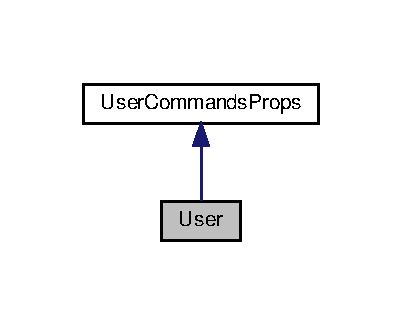
\includegraphics[width=193pt]{structUser__inherit__graph}
\end{center}
\end{figure}


Collaboration diagram for User\+:\nopagebreak
\begin{figure}[H]
\begin{center}
\leavevmode
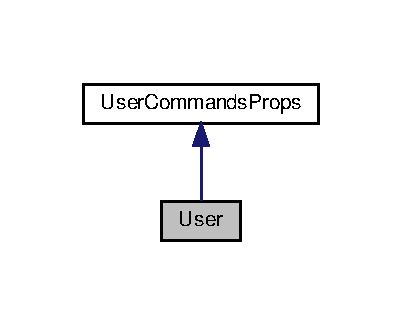
\includegraphics[width=193pt]{structUser__coll__graph}
\end{center}
\end{figure}
\subsection*{Public Attributes}
\begin{DoxyCompactItemize}
\item 
\mbox{\Hypertarget{structUser_a2f03286ef5f028e69401a8a31fc17670}\label{structUser_a2f03286ef5f028e69401a8a31fc17670}} 
bool {\bfseries logged}
\item 
\mbox{\Hypertarget{structUser_a49574651dbb03bde828ef9fb0cea17ed}\label{structUser_a49574651dbb03bde828ef9fb0cea17ed}} 
string {\bfseries uid}
\item 
\mbox{\Hypertarget{structUser_ac7f46b6a7edfa8f3044f6d50d1ec6647}\label{structUser_ac7f46b6a7edfa8f3044f6d50d1ec6647}} 
string {\bfseries gid}
\end{DoxyCompactItemize}
\subsection*{Additional Inherited Members}


The documentation for this struct was generated from the following file\+:\begin{DoxyCompactItemize}
\item 
env/index.\+h\end{DoxyCompactItemize}

\hypertarget{classuser__commands}{}\section{user\+\_\+commands Class Reference}
\label{classuser__commands}\index{user\+\_\+commands@{user\+\_\+commands}}
\subsection*{Public Member Functions}
\begin{DoxyCompactItemize}
\item 
void \hyperlink{classuser__commands_a1d8f9ded8fcaac8ed4f38b5dd1e84aa9}{login} (\hyperlink{structUserCommandsProps}{User\+Commands\+Props} props)
\begin{DoxyCompactList}\small\item\em Iniciar sesion en una particion. \end{DoxyCompactList}\item 
void \hyperlink{classuser__commands_a3465a40be3ffa4bf21758c1561b42fe5}{mkusr} (\hyperlink{structMkUserProps}{Mk\+User\+Props} props)
\begin{DoxyCompactList}\small\item\em Crea un usuario en una particion. \end{DoxyCompactList}\item 
void \hyperlink{classuser__commands_a1dc49969dc241f97636ec3680c822e3d}{rmusr} (string user)
\begin{DoxyCompactList}\small\item\em Configura el id 0 para el usuario seleccioando. \end{DoxyCompactList}\item 
void \hyperlink{classuser__commands_a9f3307fd8aa6f788c0eddeb2166c5274}{logout} ()
\begin{DoxyCompactList}\small\item\em Cerrar la sesion actual. \end{DoxyCompactList}\end{DoxyCompactItemize}


\subsection{Member Function Documentation}
\mbox{\Hypertarget{classuser__commands_a1d8f9ded8fcaac8ed4f38b5dd1e84aa9}\label{classuser__commands_a1d8f9ded8fcaac8ed4f38b5dd1e84aa9}} 
\index{user\+\_\+commands@{user\+\_\+commands}!login@{login}}
\index{login@{login}!user\+\_\+commands@{user\+\_\+commands}}
\subsubsection{\texorpdfstring{login()}{login()}}
{\footnotesize\ttfamily void user\+\_\+commands\+::login (\begin{DoxyParamCaption}\item[{\hyperlink{structUserCommandsProps}{User\+Commands\+Props}}]{props }\end{DoxyParamCaption})}



Iniciar sesion en una particion. 

Login 
\begin{DoxyParams}{Parameters}
{\em \{user\+\_\+commands\}} & user\+\_\+data \\
\hline
\end{DoxyParams}
\mbox{\Hypertarget{classuser__commands_a9f3307fd8aa6f788c0eddeb2166c5274}\label{classuser__commands_a9f3307fd8aa6f788c0eddeb2166c5274}} 
\index{user\+\_\+commands@{user\+\_\+commands}!logout@{logout}}
\index{logout@{logout}!user\+\_\+commands@{user\+\_\+commands}}
\subsubsection{\texorpdfstring{logout()}{logout()}}
{\footnotesize\ttfamily void user\+\_\+commands\+::logout (\begin{DoxyParamCaption}{ }\end{DoxyParamCaption})}



Cerrar la sesion actual. 

Logout \mbox{\Hypertarget{classuser__commands_a3465a40be3ffa4bf21758c1561b42fe5}\label{classuser__commands_a3465a40be3ffa4bf21758c1561b42fe5}} 
\index{user\+\_\+commands@{user\+\_\+commands}!mkusr@{mkusr}}
\index{mkusr@{mkusr}!user\+\_\+commands@{user\+\_\+commands}}
\subsubsection{\texorpdfstring{mkusr()}{mkusr()}}
{\footnotesize\ttfamily void user\+\_\+commands\+::mkusr (\begin{DoxyParamCaption}\item[{\hyperlink{structMkUserProps}{Mk\+User\+Props}}]{props }\end{DoxyParamCaption})}



Crea un usuario en una particion. 

Crear usuario 
\begin{DoxyParams}{Parameters}
{\em \{user\+\_\+commands\}} & user\+\_\+data \\
\hline
\end{DoxyParams}
\mbox{\Hypertarget{classuser__commands_a1dc49969dc241f97636ec3680c822e3d}\label{classuser__commands_a1dc49969dc241f97636ec3680c822e3d}} 
\index{user\+\_\+commands@{user\+\_\+commands}!rmusr@{rmusr}}
\index{rmusr@{rmusr}!user\+\_\+commands@{user\+\_\+commands}}
\subsubsection{\texorpdfstring{rmusr()}{rmusr()}}
{\footnotesize\ttfamily void user\+\_\+commands\+::rmusr (\begin{DoxyParamCaption}\item[{string}]{user }\end{DoxyParamCaption})}



Configura el id 0 para el usuario seleccioando. 

Borrar usuario 
\begin{DoxyParams}{Parameters}
{\em \{user\+\_\+commands\}} & user\+\_\+data \\
\hline
\end{DoxyParams}


The documentation for this class was generated from the following files\+:\begin{DoxyCompactItemize}
\item 
users/index.\+h\item 
users/index.\+cpp\end{DoxyCompactItemize}

\hypertarget{structUserCommandsProps}{}\section{User\+Commands\+Props Struct Reference}
\label{structUserCommandsProps}\index{User\+Commands\+Props@{User\+Commands\+Props}}


Inheritance diagram for User\+Commands\+Props\+:\nopagebreak
\begin{figure}[H]
\begin{center}
\leavevmode
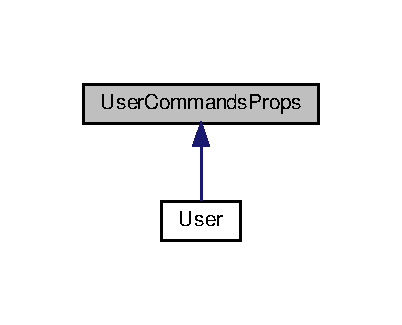
\includegraphics[width=193pt]{structUserCommandsProps__inherit__graph}
\end{center}
\end{figure}
\subsection*{Public Member Functions}
\begin{DoxyCompactItemize}
\item 
\mbox{\Hypertarget{structUserCommandsProps_a4740b3e981ed7efa3acd981a47c98191}\label{structUserCommandsProps_a4740b3e981ed7efa3acd981a47c98191}} 
void {\bfseries set\+\_\+prop} (string value, string key)
\end{DoxyCompactItemize}
\subsection*{Public Attributes}
\begin{DoxyCompactItemize}
\item 
\mbox{\Hypertarget{structUserCommandsProps_a4dbe9ca2f3589e635ffb110c5a57268f}\label{structUserCommandsProps_a4dbe9ca2f3589e635ffb110c5a57268f}} 
string {\bfseries user}
\item 
\mbox{\Hypertarget{structUserCommandsProps_a673b028f7b238168b76ff117e1630768}\label{structUserCommandsProps_a673b028f7b238168b76ff117e1630768}} 
string {\bfseries pwd}
\item 
\mbox{\Hypertarget{structUserCommandsProps_a7dfa262b7f34e98fa0c57f4a9a739675}\label{structUserCommandsProps_a7dfa262b7f34e98fa0c57f4a9a739675}} 
string {\bfseries grp}
\item 
\mbox{\Hypertarget{structUserCommandsProps_a4585588abc2524f941f500e44c6f241c}\label{structUserCommandsProps_a4585588abc2524f941f500e44c6f241c}} 
string {\bfseries id}
\end{DoxyCompactItemize}


The documentation for this struct was generated from the following file\+:\begin{DoxyCompactItemize}
\item 
users/index.\+h\end{DoxyCompactItemize}

\hypertarget{structUserOrGroup}{}\section{User\+Or\+Group Struct Reference}
\label{structUserOrGroup}\index{User\+Or\+Group@{User\+Or\+Group}}
\subsection*{Public Attributes}
\begin{DoxyCompactItemize}
\item 
\mbox{\Hypertarget{structUserOrGroup_a0e90e628f1aebf94b62b647b39890881}\label{structUserOrGroup_a0e90e628f1aebf94b62b647b39890881}} 
string {\bfseries uid}
\item 
\mbox{\Hypertarget{structUserOrGroup_a39ac76cda383b9db38845bc0903b84f5}\label{structUserOrGroup_a39ac76cda383b9db38845bc0903b84f5}} 
string {\bfseries type}
\item 
\mbox{\Hypertarget{structUserOrGroup_ad5c8dbb858d34ae023b3e2addd511978}\label{structUserOrGroup_ad5c8dbb858d34ae023b3e2addd511978}} 
string {\bfseries name}
\item 
\mbox{\Hypertarget{structUserOrGroup_a95ab040240784fe1ed5f19612f834543}\label{structUserOrGroup_a95ab040240784fe1ed5f19612f834543}} 
string {\bfseries pwd}
\item 
\mbox{\Hypertarget{structUserOrGroup_ad089ab60be3f1f00d68303f80dc0fe42}\label{structUserOrGroup_ad089ab60be3f1f00d68303f80dc0fe42}} 
string {\bfseries grp}
\end{DoxyCompactItemize}


The documentation for this struct was generated from the following file\+:\begin{DoxyCompactItemize}
\item 
users/index.\+h\end{DoxyCompactItemize}

\hypertarget{structyy__buffer__state}{}\section{yy\+\_\+buffer\+\_\+state Struct Reference}
\label{structyy__buffer__state}\index{yy\+\_\+buffer\+\_\+state@{yy\+\_\+buffer\+\_\+state}}
\subsection*{Public Attributes}
\begin{DoxyCompactItemize}
\item 
\mbox{\Hypertarget{structyy__buffer__state_a4360acfb226a1fc240ab2be17dd6beda}\label{structyy__buffer__state_a4360acfb226a1fc240ab2be17dd6beda}} 
F\+I\+LE $\ast$ {\bfseries yy\+\_\+input\+\_\+file}
\item 
\mbox{\Hypertarget{structyy__buffer__state_a0d25458e69eb22207fc633a1255d099d}\label{structyy__buffer__state_a0d25458e69eb22207fc633a1255d099d}} 
char $\ast$ {\bfseries yy\+\_\+ch\+\_\+buf}
\item 
\mbox{\Hypertarget{structyy__buffer__state_a8435c3f786bbb55d21d0174e4cfc22a0}\label{structyy__buffer__state_a8435c3f786bbb55d21d0174e4cfc22a0}} 
char $\ast$ {\bfseries yy\+\_\+buf\+\_\+pos}
\item 
\mbox{\Hypertarget{structyy__buffer__state_a451d39697f006f3922c1f43cf79286b4}\label{structyy__buffer__state_a451d39697f006f3922c1f43cf79286b4}} 
int {\bfseries yy\+\_\+buf\+\_\+size}
\item 
\mbox{\Hypertarget{structyy__buffer__state_a06406208824817acfec2183b79080945}\label{structyy__buffer__state_a06406208824817acfec2183b79080945}} 
int {\bfseries yy\+\_\+n\+\_\+chars}
\item 
\mbox{\Hypertarget{structyy__buffer__state_a80ce2431c70dc4f89ced487f18449465}\label{structyy__buffer__state_a80ce2431c70dc4f89ced487f18449465}} 
int {\bfseries yy\+\_\+is\+\_\+our\+\_\+buffer}
\item 
\mbox{\Hypertarget{structyy__buffer__state_abf5c70eea75581b58c0ee7bd31b14490}\label{structyy__buffer__state_abf5c70eea75581b58c0ee7bd31b14490}} 
int {\bfseries yy\+\_\+is\+\_\+interactive}
\item 
\mbox{\Hypertarget{structyy__buffer__state_a9d60c60af6e1a6f69de16871fd64f85f}\label{structyy__buffer__state_a9d60c60af6e1a6f69de16871fd64f85f}} 
int {\bfseries yy\+\_\+at\+\_\+bol}
\item 
int \hyperlink{structyy__buffer__state_a818e94bc9c766e683c60df1e9fd01199}{yy\+\_\+bs\+\_\+lineno}
\item 
int \hyperlink{structyy__buffer__state_a10c4fcd8be759e6bf11e6d3e8cdb0307}{yy\+\_\+bs\+\_\+column}
\item 
\mbox{\Hypertarget{structyy__buffer__state_a63d2afbb1d79a3fc63df9e12626f827d}\label{structyy__buffer__state_a63d2afbb1d79a3fc63df9e12626f827d}} 
int {\bfseries yy\+\_\+fill\+\_\+buffer}
\item 
\mbox{\Hypertarget{structyy__buffer__state_a70fd925d37a2f0454fbd0def675d106c}\label{structyy__buffer__state_a70fd925d37a2f0454fbd0def675d106c}} 
int {\bfseries yy\+\_\+buffer\+\_\+status}
\end{DoxyCompactItemize}


\subsection{Member Data Documentation}
\mbox{\Hypertarget{structyy__buffer__state_a10c4fcd8be759e6bf11e6d3e8cdb0307}\label{structyy__buffer__state_a10c4fcd8be759e6bf11e6d3e8cdb0307}} 
\index{yy\+\_\+buffer\+\_\+state@{yy\+\_\+buffer\+\_\+state}!yy\+\_\+bs\+\_\+column@{yy\+\_\+bs\+\_\+column}}
\index{yy\+\_\+bs\+\_\+column@{yy\+\_\+bs\+\_\+column}!yy\+\_\+buffer\+\_\+state@{yy\+\_\+buffer\+\_\+state}}
\subsubsection{\texorpdfstring{yy\+\_\+bs\+\_\+column}{yy\_bs\_column}}
{\footnotesize\ttfamily int yy\+\_\+buffer\+\_\+state\+::yy\+\_\+bs\+\_\+column}

The column count. \mbox{\Hypertarget{structyy__buffer__state_a818e94bc9c766e683c60df1e9fd01199}\label{structyy__buffer__state_a818e94bc9c766e683c60df1e9fd01199}} 
\index{yy\+\_\+buffer\+\_\+state@{yy\+\_\+buffer\+\_\+state}!yy\+\_\+bs\+\_\+lineno@{yy\+\_\+bs\+\_\+lineno}}
\index{yy\+\_\+bs\+\_\+lineno@{yy\+\_\+bs\+\_\+lineno}!yy\+\_\+buffer\+\_\+state@{yy\+\_\+buffer\+\_\+state}}
\subsubsection{\texorpdfstring{yy\+\_\+bs\+\_\+lineno}{yy\_bs\_lineno}}
{\footnotesize\ttfamily int yy\+\_\+buffer\+\_\+state\+::yy\+\_\+bs\+\_\+lineno}

The line count. 

The documentation for this struct was generated from the following files\+:\begin{DoxyCompactItemize}
\item 
lang/scanner.\+cpp\item 
lang/scanner.\+h\end{DoxyCompactItemize}

\hypertarget{structyy__trans__info}{}\section{yy\+\_\+trans\+\_\+info Struct Reference}
\label{structyy__trans__info}\index{yy\+\_\+trans\+\_\+info@{yy\+\_\+trans\+\_\+info}}
\subsection*{Public Attributes}
\begin{DoxyCompactItemize}
\item 
\mbox{\Hypertarget{structyy__trans__info_a5c9f61e770deef50bd4e697310342fe9}\label{structyy__trans__info_a5c9f61e770deef50bd4e697310342fe9}} 
flex\+\_\+int32\+\_\+t {\bfseries yy\+\_\+verify}
\item 
\mbox{\Hypertarget{structyy__trans__info_ae0715250c2bef261e596e77e0030f13e}\label{structyy__trans__info_ae0715250c2bef261e596e77e0030f13e}} 
flex\+\_\+int32\+\_\+t {\bfseries yy\+\_\+nxt}
\end{DoxyCompactItemize}


The documentation for this struct was generated from the following file\+:\begin{DoxyCompactItemize}
\item 
lang/scanner.\+cpp\end{DoxyCompactItemize}

\hypertarget{unionyyalloc}{}\section{yyalloc Union Reference}
\label{unionyyalloc}\index{yyalloc@{yyalloc}}


Collaboration diagram for yyalloc\+:\nopagebreak
\begin{figure}[H]
\begin{center}
\leavevmode
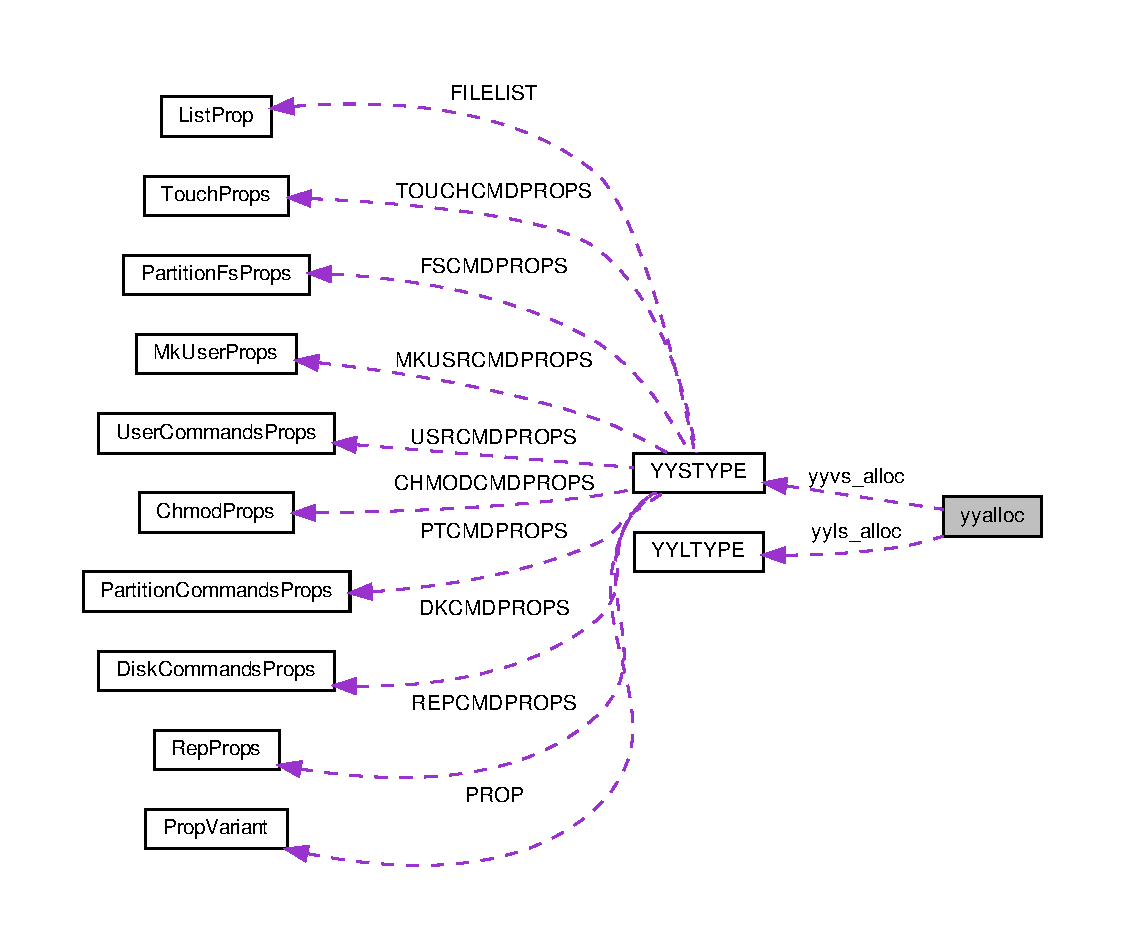
\includegraphics[width=350pt]{unionyyalloc__coll__graph}
\end{center}
\end{figure}
\subsection*{Public Attributes}
\begin{DoxyCompactItemize}
\item 
\mbox{\Hypertarget{unionyyalloc_a4800e0520a89a4789afa7b5d82197e65}\label{unionyyalloc_a4800e0520a89a4789afa7b5d82197e65}} 
yytype\+\_\+int16 {\bfseries yyss\+\_\+alloc}
\item 
\mbox{\Hypertarget{unionyyalloc_a9326f4fdc6f737a929444427836d8928}\label{unionyyalloc_a9326f4fdc6f737a929444427836d8928}} 
\hyperlink{unionYYSTYPE}{Y\+Y\+S\+T\+Y\+PE} {\bfseries yyvs\+\_\+alloc}
\item 
\mbox{\Hypertarget{unionyyalloc_a542e43248e6afac9af342c2f4e3162fc}\label{unionyyalloc_a542e43248e6afac9af342c2f4e3162fc}} 
\hyperlink{structYYLTYPE}{Y\+Y\+L\+T\+Y\+PE} {\bfseries yyls\+\_\+alloc}
\end{DoxyCompactItemize}


The documentation for this union was generated from the following file\+:\begin{DoxyCompactItemize}
\item 
lang/parser.\+cpp\end{DoxyCompactItemize}

\hypertarget{structYYLTYPE}{}\section{Y\+Y\+L\+T\+Y\+PE Struct Reference}
\label{structYYLTYPE}\index{Y\+Y\+L\+T\+Y\+PE@{Y\+Y\+L\+T\+Y\+PE}}
\subsection*{Public Attributes}
\begin{DoxyCompactItemize}
\item 
\mbox{\Hypertarget{structYYLTYPE_a50ad3435eaea74bcab6f1ae5fbaefd89}\label{structYYLTYPE_a50ad3435eaea74bcab6f1ae5fbaefd89}} 
int {\bfseries first\+\_\+line}
\item 
\mbox{\Hypertarget{structYYLTYPE_a3a556533babab1b9066fa9bdbb809210}\label{structYYLTYPE_a3a556533babab1b9066fa9bdbb809210}} 
int {\bfseries first\+\_\+column}
\item 
\mbox{\Hypertarget{structYYLTYPE_a3075f2bc3448df5d2a9f16d22bff2cc1}\label{structYYLTYPE_a3075f2bc3448df5d2a9f16d22bff2cc1}} 
int {\bfseries last\+\_\+line}
\item 
\mbox{\Hypertarget{structYYLTYPE_acf87f8c98686f286eaf700c4b62157b2}\label{structYYLTYPE_acf87f8c98686f286eaf700c4b62157b2}} 
int {\bfseries last\+\_\+column}
\end{DoxyCompactItemize}


The documentation for this struct was generated from the following files\+:\begin{DoxyCompactItemize}
\item 
lang/parser.\+cpp\item 
lang/parser.\+h\end{DoxyCompactItemize}

\hypertarget{unionYYSTYPE}{}\section{Y\+Y\+S\+T\+Y\+PE Union Reference}
\label{unionYYSTYPE}\index{Y\+Y\+S\+T\+Y\+PE@{Y\+Y\+S\+T\+Y\+PE}}


Collaboration diagram for Y\+Y\+S\+T\+Y\+PE\+:\nopagebreak
\begin{figure}[H]
\begin{center}
\leavevmode
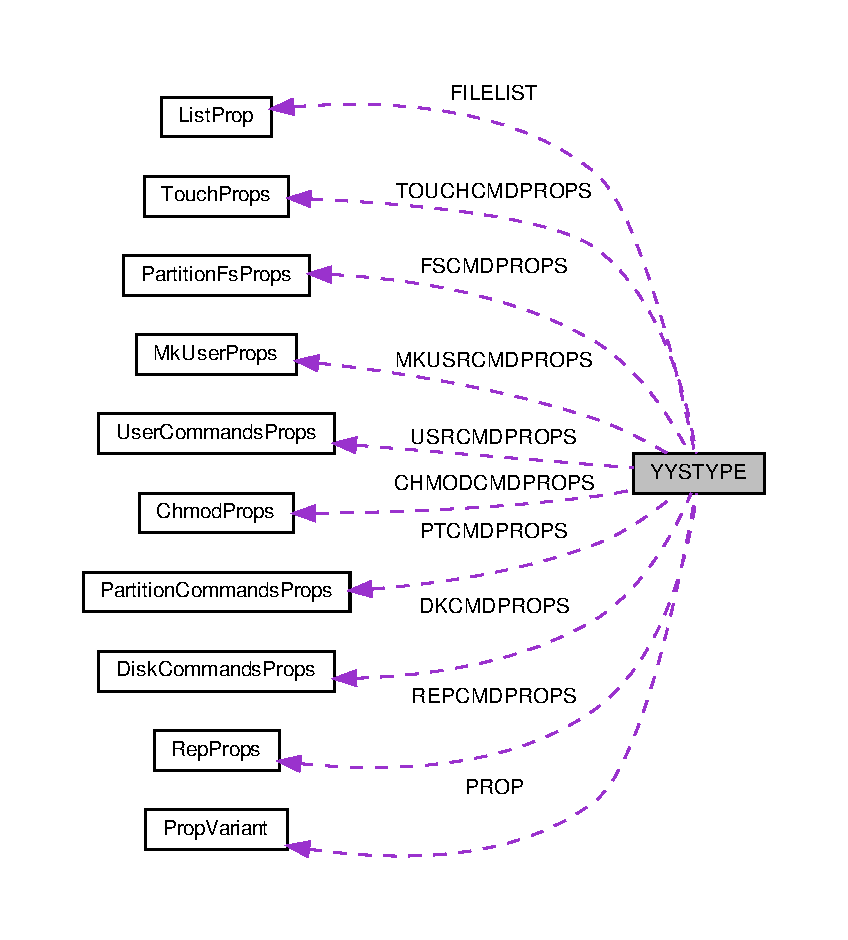
\includegraphics[width=350pt]{unionYYSTYPE__coll__graph}
\end{center}
\end{figure}
\subsection*{Public Attributes}
\begin{DoxyCompactItemize}
\item 
\mbox{\Hypertarget{unionYYSTYPE_aee5c8cb30473950cb4797e4f16692e13}\label{unionYYSTYPE_aee5c8cb30473950cb4797e4f16692e13}} 
struct \hyperlink{structPartitionCommandsProps}{Partition\+Commands\+Props} $\ast$ {\bfseries P\+T\+C\+M\+D\+P\+R\+O\+PS}
\item 
\mbox{\Hypertarget{unionYYSTYPE_a1f8bf7be4e2a8803f1b9d56a7091e699}\label{unionYYSTYPE_a1f8bf7be4e2a8803f1b9d56a7091e699}} 
struct \hyperlink{structDiskCommandsProps}{Disk\+Commands\+Props} $\ast$ {\bfseries D\+K\+C\+M\+D\+P\+R\+O\+PS}
\item 
\mbox{\Hypertarget{unionYYSTYPE_a17a0a65338bd94f30a3b3a98b96196dc}\label{unionYYSTYPE_a17a0a65338bd94f30a3b3a98b96196dc}} 
struct \hyperlink{structPartitionFsProps}{Partition\+Fs\+Props} $\ast$ {\bfseries F\+S\+C\+M\+D\+P\+R\+O\+PS}
\item 
\mbox{\Hypertarget{unionYYSTYPE_aa82020c9db3f6c43a11ccc8e5f190788}\label{unionYYSTYPE_aa82020c9db3f6c43a11ccc8e5f190788}} 
struct \hyperlink{structUserCommandsProps}{User\+Commands\+Props} $\ast$ {\bfseries U\+S\+R\+C\+M\+D\+P\+R\+O\+PS}
\item 
\mbox{\Hypertarget{unionYYSTYPE_a37a52627f8f812d79a7c32fee6f8cad2}\label{unionYYSTYPE_a37a52627f8f812d79a7c32fee6f8cad2}} 
struct \hyperlink{structMkUserProps}{Mk\+User\+Props} $\ast$ {\bfseries M\+K\+U\+S\+R\+C\+M\+D\+P\+R\+O\+PS}
\item 
\mbox{\Hypertarget{unionYYSTYPE_a899d0cb6dc31f22e1fd2ff2792136782}\label{unionYYSTYPE_a899d0cb6dc31f22e1fd2ff2792136782}} 
struct \hyperlink{structChmodProps}{Chmod\+Props} $\ast$ {\bfseries C\+H\+M\+O\+D\+C\+M\+D\+P\+R\+O\+PS}
\item 
\mbox{\Hypertarget{unionYYSTYPE_a4e86ad2aba2902edbfb7ca0687d40231}\label{unionYYSTYPE_a4e86ad2aba2902edbfb7ca0687d40231}} 
struct \hyperlink{structTouchProps}{Touch\+Props} $\ast$ {\bfseries T\+O\+U\+C\+H\+C\+M\+D\+P\+R\+O\+PS}
\item 
\mbox{\Hypertarget{unionYYSTYPE_ac360f0342757e36c16407a4d39ecc914}\label{unionYYSTYPE_ac360f0342757e36c16407a4d39ecc914}} 
struct \hyperlink{structRepProps}{Rep\+Props} $\ast$ {\bfseries R\+E\+P\+C\+M\+D\+P\+R\+O\+PS}
\item 
\mbox{\Hypertarget{unionYYSTYPE_ace81d82c79a18e3aa42d859a06d26412}\label{unionYYSTYPE_ace81d82c79a18e3aa42d859a06d26412}} 
struct \hyperlink{structListProp}{List\+Prop} $\ast$ {\bfseries F\+I\+L\+E\+L\+I\+ST}
\item 
\mbox{\Hypertarget{unionYYSTYPE_a65f6ba013618ca3d5a033e1f94a1969b}\label{unionYYSTYPE_a65f6ba013618ca3d5a033e1f94a1969b}} 
struct \hyperlink{structPropVariant}{Prop\+Variant} {\bfseries P\+R\+OP}
\item 
\mbox{\Hypertarget{unionYYSTYPE_a61a79fb526a85cd54af103786554fee6}\label{unionYYSTYPE_a61a79fb526a85cd54af103786554fee6}} 
char $\ast$ {\bfseries T\+E\+XT}
\end{DoxyCompactItemize}


The documentation for this union was generated from the following files\+:\begin{DoxyCompactItemize}
\item 
lang/parser.\+cpp\item 
lang/parser.\+h\end{DoxyCompactItemize}

%--- End generated contents ---

% Index
\backmatter
\newpage
\phantomsection
\clearemptydoublepage
\addcontentsline{toc}{chapter}{Index}
\printindex

\end{document}
